%%%%%%%%%%%%%%%%%%%%%%%%%%%%%%%%%%%%%%%%%%%%%%%%%%%%%%%%%%%%%%%%%%%%%%%%%%%
%%                                                                       %%
%%     LaTeX + CTeX 《应用概率统计》论文模板, 只针对 A4 纸英文稿.        %%
%%                                                                       %%
%%%%%%%%%%%%%%%%%%%%%%%%%%%%%%%%%%%%%%%%%%%%%%%%%%%%%%%%%%%%%%%%%%%%%%%%%%%

%%%%%%%%%%%%%%%%%%%%%%%%%%%%%%%%%%%%%%%%%%%%%%%%%%%%%%%%%%%%%%%%
%            英文稿 文章模板:A4 纸, 五号字, 单列              %
%%%%%%%%%%%%%%%%%%%%%%%%%%%%%%%%%%%%%%%%%%%%%%%%%%%%%%%%%%%%%%%%
\documentclass[a4paper,c5size,onecolumn,twoside,nocap,English]{APSart}
\begin{document}

\setcounter{page}{1}

%%%%%%%%%%%%%%%%%%%%%%%%%%%%%%%%%%%%%%%%%%%%%%%%%%%%%%%%%%%%%%%%
%%------------------ 编辑部提供的信息 ------------------------%%
%%%%%%%%%%%%%%%%%%%%%%%%%%%%%%%%%%%%%%%%%%%%%%%%%%%%%%%%%%%%%%%%
\newcommand{\pubvol}{xx}         % 卷号
\newcommand{\enpubvol}{xx}       % 卷号
\newcommand{\pubno}{x}           % 期号
\newcommand{\enpubno}{x}         % 期号
\newcommand{\pubyear}{20xx}      % 出版年份
\newcommand{\enpubyear}{20xx}    % 出版年份
\newcommand{\pubmonth}{xx}       % 出版月份
\newcommand{\enpubmonth}{xx}     % 出版月份
\newcommand{\ksym}{xxx}          % 开始页码
\newcommand{\jsym}{xxx}          % 结束页码
\newcommand{\receivedate}{Received Month Date, Year.} % 论文收到日期
\newcommand{\modifydate}{Revised Month Date, Year.} % 论文修改日期
\newcommand{\doino}{10.3969/j.issn.1001-4268.20xx.0x.0xx} % doi号
%%
%%%%%%%%%%%%%%%%%%%%%%%%%%%%%%%%%%%%%%%%%%%%%%%%%%%%%%%%%%%%%%%%
%%-------------------- 作者提供的信息 ------------------------%%
%%%%%%%%%%%%%%%%%%%%%%%%%%%%%%%%%%%%%%%%%%%%%%%%%%%%%%%%%%%%%%%%
\newcommand{\cnfirstauthor}{第一作者姓名}
\newcommand{\cnsecondauthor}{第二作者姓名}
\newcommand{\cnfirstinst}{第一作者单位(到部门), 省市, 邮政编码}
\newcommand{\cnsecondinst}{第二作者单位(到部门), 省市, 邮政编码}
\newcommand{\cntitle}{论文题目}
\newcommand{\cnkeywords}{关键词1; 关键词2; ......}
\newcommand{\cnclassno}{O212.xx} % 中图分类号
%%
\newcommand{\runenauthors}{FIRST N., SECOND N.} %超过两个作者的请用:First Name et al.
\newcommand{\runentitle}{English Title Abbreviation} %英文标题缩写, 用于放在页眉
\newcommand{\enfirstauthor}{FIRST Name}
\newcommand{\ensecondauthor}{SECOND Name}
\newcommand{\enfirstinst}{First Author's Working Unit $($Up to Department$)$, Province, 
Zip Code, China}
\newcommand{\ensecondinst}{Second Author's Working Unit $($Up to Department$)$, Province, 
Zip Code, China}
\newcommand{\entitle}{English Title}
\newcommand{\enkeywords}{keyword 1; keyword 2; ......}
\newcommand{\amsno}{62Nxx} % AMS Subject Claassification
%%
%% 中文摘要
\newcommand{\cnabstract}{摘要内容.}
%% 英文摘要
\newcommand{\enabstract}{The abstract comes here.}
\newcommand{\fundinfo}{The project was supported by XXXX foundation (12345678).}
\newcommand{\authorsinfo}{\textbf{作者信息}:~ %% 使用中文
第一作者(出生时间--),~性别,~职称,~主要研究方向:~xxxxxx,~E-mail:xxxxx@xxxx.xxx.xx~;
第二作者(出生时间--):~性别,~职称,~主要研究方向:~xxxxxx,~E-mail:xxxxx@xxxx.xxx.xx~.}

%%%%%%%%%%%%%%%%%%%%%%%%%%%%%%%%%%%%%%%%%%%%%%%%%%%%%%%%%%%%%%%%
%        文章正文                                              %
%%%%%%%%%%%%%%%%%%%%%%%%%%%%%%%%%%%%%%%%%%%%%%%%%%%%%%%%%%%%%%%%

\title{\Large\bf{\entitle}
\thanks{\scriptsize{\fundinfo}}
}
%%%%%%%%%%%%%%%%%%%%%%%%%%%%%%%%%%%%%%%%%%%%%%%%%%%%%%%%%%%%%%%%
% 作者姓名与单位 : 三种形式中选一种
% 后面中文摘要中的名字和单位同样处理
% ---------------------
% 第一种形式: 单一作者
% ---------------------
%\author{\textrm{\enfirstauthor}\\[-2pt]
%(\textit{\zihao{-5}\enfirstinst})}

% ---------------------
% 第二种形式: 同一单位 多个作者 -- 名字左右并列,
% ---------------------
\author{\textrm{\enfirstauthor\hy\hy\hy\ensecondauthor}\\[-2pt]
(\textit{\zihao{-5}\enfirstinst})}

% ---------------------
% 第三种形式: 不同单位 多个作者 -- 名字与单位上下并列
% ---------------------
%\author{\textrm{\enfirstauthor}\\[-2pt]
%(\textit{\zihao{-5}\enfirstinst})\\[1pt]
%\textrm{\ensecondauthor}\\[-2pt]
%(\textit{\zihao{-5}\ensecondinst})}
%%%%%%%%%%%%%%%%%%%%%%%%%%%%%%%%%%%%%%%%%%%%%%%%%%%%%%%%%%%%%%%%

\date{} % 这一行用来去掉默认的日期显示
\maketitle
\vspace{-6mm}
%%%%%%%%%%%%%%%%%%%%%%%%%%%%%%%%%%%%%%%%%%%%%%%%%%%%%%%%%%%%%%%%
%  英文文摘要
%%%%%%%%%%%%%%%%%%%%%%%%%%%%%%%%%%%%%%%%%%%%%%%%%%%%%%%%%%%%%%%%
\begin{center}
\begin{minipage}[c]{14cm}
\zihao{-5}
\hspace{2\ccwd}\textbf{Abstract:}\quad\enabstract\\
\mbox{}\hspace{2\ccwd}\textbf{Keywords:}\quad\enkeywords\\
\mbox{}\hspace{2\ccwd}\textbf{2010 Mathematics Subject Classification:}\quad\amsno
\end{minipage}
\end{center}
\footnote[0]{\scriptsize{\receivedate~~\modifydate\\
\authorsinfo}}\vspace{-1em}

%%%%%%%%%%%%%%%%%%%%%%%%%%%%%%%%%%%%%%%%%%%%%%%%%%%%%%%%%%%%%%%%
%  正文由此开始
%%%%%%%%%%%%%%%%%%%%%%%%%%%%%%%%%%%%%%%%%%%%%%%%%%%%%%%%%%%%%%%%

%%%%%%%%%%%%%%%%%%%%%%%%%%%%%%%%%%%% %%%%%%%%%%%%%%%%%%%%%%%%%%%%
\section{Introduction}
%%%%%%%%%%%%%%%%%%%%%%%%%%%%%%%%%%%%%%%%%%%%%%%%%%%%%%%%%%%%%%%%

This a \LaTeX{} template specially designed for Chinese Journal of Applied Probability and Statistics.

%%%%%%%%%%%%%%%%%%%%%%%%%%%%%%%%%%%% %%%%%%%%%%%%%%%%%%%%%%%%%%%%
\section{Common environments in \LaTeX{}}
%%%%%%%%%%%%%%%%%%%%%%%%%%%%%%%%%%%%%%%%%%%%%%%%%%%%%%%%%%%%%%%%

\subsection{Classification}

See the four categories in the Chinese version.

\subsection{Examples}

Here are some examples of formulae, tables, figure insertions, citations for your reference.
\begin{equation}\label{eq:1}
\left\{ \begin{aligned}
         \pi &= 3.141\cdots \\
     \sqrt{2}&=1.414\cdots
         \end{aligned} \right.
\end{equation}
\begin{align}
	\pi &= 3.1415926\cdots \nonumber \\
		&\approx  3.14.
\end{align}

\begin{table}[htbp]
\centering\zihao{5}
\caption{Table with horizontal and vertical lines\label{table:1}}
\vskip2mm
\begin{tabular}{r|l||c|rrr|c|c}
\toprule
Positiion & Club & Games & W & T & L & Goals & Points \\ [0.5ex]
\midrule
1 & Amesville Rockets & 33 & 19 & 13 & 1 & 66:31& 51:15\\
2 & Borden Comets & 33 & 18 & 9 & 6 &65:37 & 45:21\\ \hline
$\vdots$& $\vdots$ &&&&& &$\vdots$\\ \hline
17 & Quincy Giants & 33 & 7 & 5 & 21 & 40:89 &19:47\\ \hline
18 & Arlson Regulars & 33 & 3 & 11 &19 & 37:74 &17:49 \\
\bottomrule
\end{tabular}
\end{table}

\begin{figure}[htbp]
\centering
\includegraphics[width=10cm,height=3cm]{figs/sin}
\caption{A floating figure\label{fig:fig4}}
\end{figure}

\begin{figure}[htbp]
\begin{minipage}[t]{0.45\linewidth}
\centering
\includegraphics[width=6cm,height=3cm]{figs/sin}
\caption{The first subfigure\label{fig:float2-1}}
\end{minipage}
\hfill
\begin{minipage}[t]{0.5\linewidth}
\centering
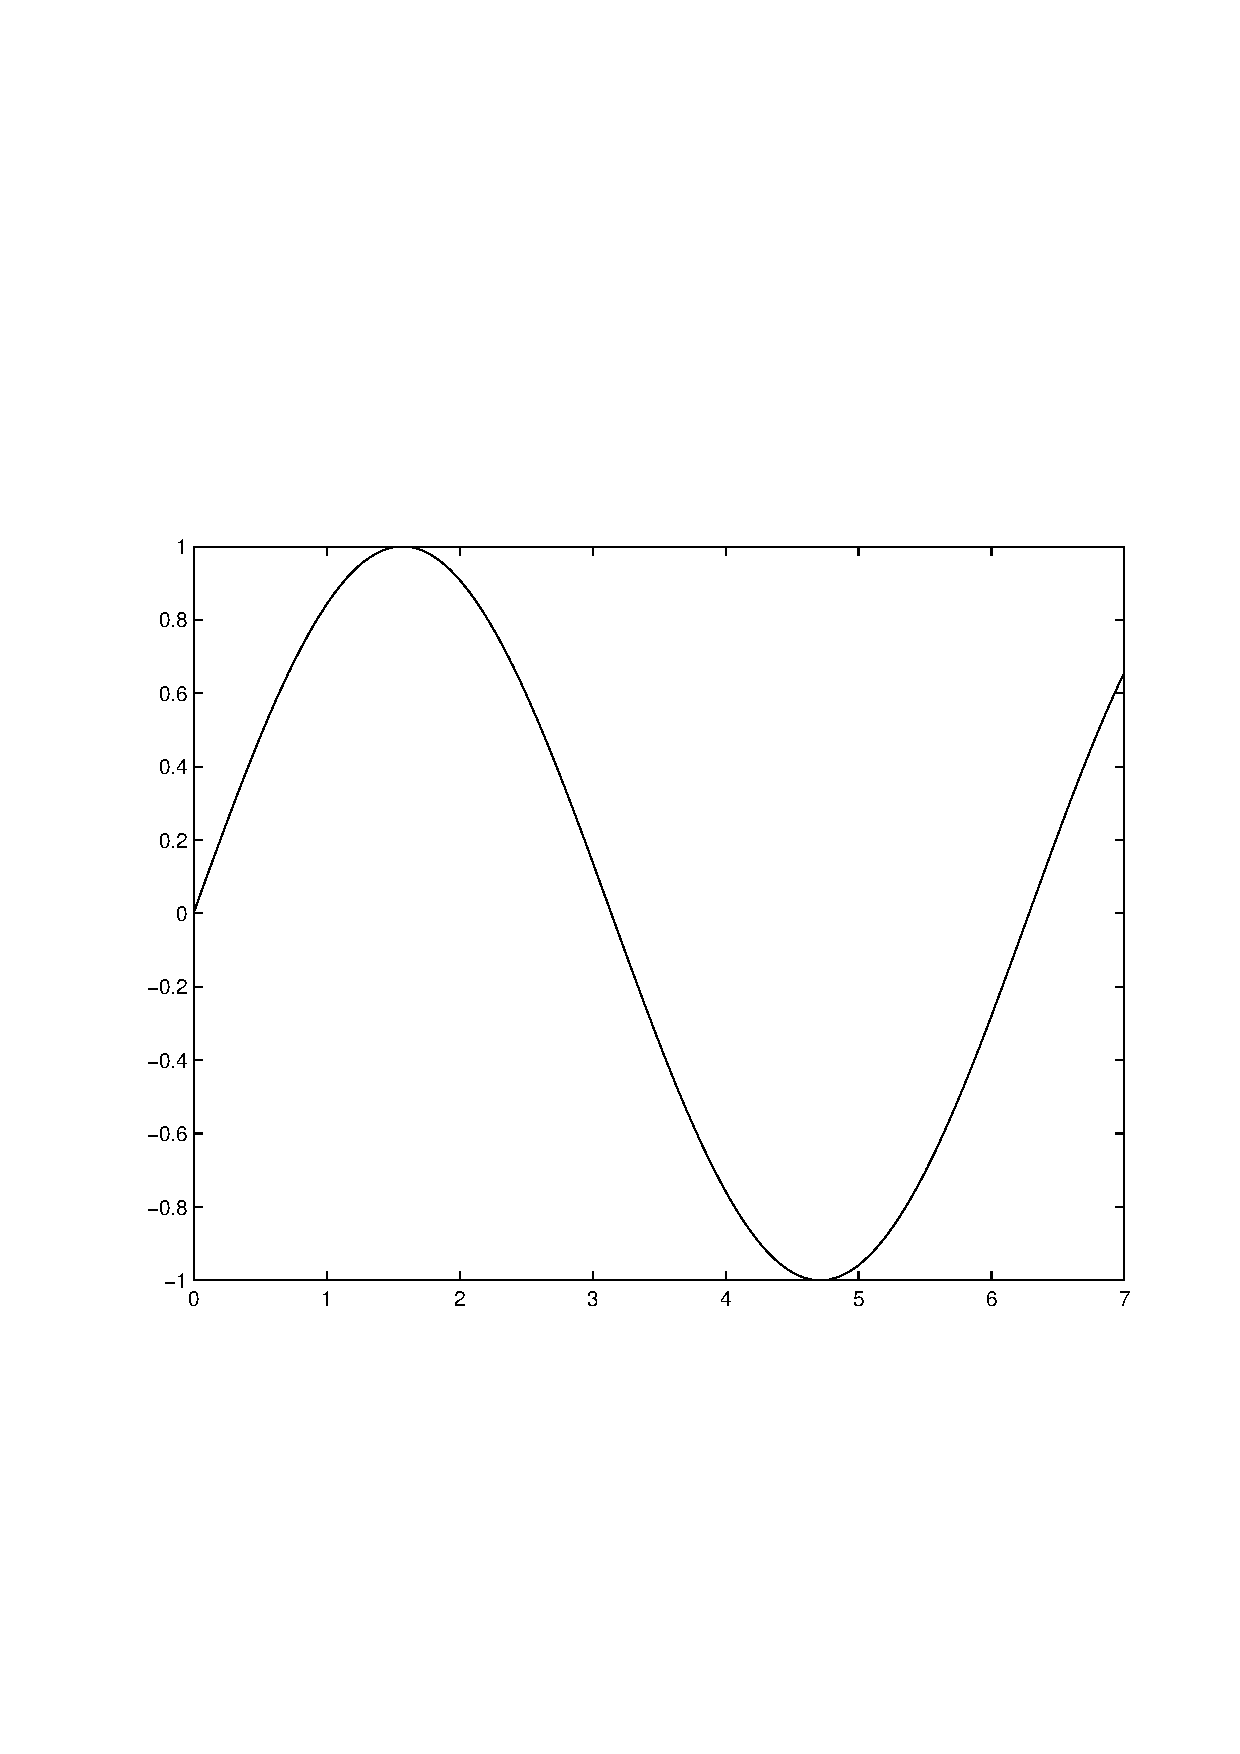
\includegraphics[width=5cm,height=3cm]{figs/fig}
\caption{The second subfigure\label{fig:float2-2}}
\end{minipage}
\end{figure}

\begin{definition}
This the definition... .
\end{definition}

\begin{lemma}
Here is the content of the lemma.
\end{lemma}

\begin{theorem}\label{thm-1}
Here is the content of Theorem \ref{thm-1}.
\end{theorem}

\begin{theorem}[Uniqueness criterion]\label{thm-2}
Here is the content of Theorem \ref{thm-2}.
\end{theorem}

\begin{proof}
Here comes the proof of the theorem.
\end{proof}

\begin{corollary}
Here is the content of the corollary.
\end{corollary}

\begin{proposition}
This is a proposition.
\end{proposition}


Now comes some examples about citation:

\begin{example}
See Formula \eqref{eq:1} on page \pageref{eq:1}.
\end{example}

\begin{example}
See Table \ref{table:1} on page \pageref{table:1}.
\end{example}

\begin{example}
See Figure \ref{fig:float2-1} on page \pageref{fig:float2-1}.
\end{example}

\begin{example}
See Theorem \ref{thm-1} on page \pageref{thm-1}.
\end{example}

\begin{example}
Please refer to \ncite{Dengjs01}, Deng\ucite{Dengjs01} or other versions with remarks such as \rcite{Dengjs01}{page 186}, \rcite{Dengjs01}{Chap. 3, \S 2, Theorems 3 and 4}.
\end{example}

\begin{example}
We use the form of \ncite{Art} for the article format, \ncite{Book} for the book format, \ncite{Book-part} for the chapter of book format and \cite{Conference} for articles in a collection of a conference.
\end{example}

%%%%%%%%%%%%%%%%%%%%%%%%%%%%%%%%%%%%%%%%%%%%%%%%%%%%%%%%%%%%%%%%
\section{Remarks}
%%%%%%%%%%%%%%%%%%%%%%%%%%%%%%%%%%%%%%%%%%%%%%%%%%%%%%%%%%%%%%%%

\begin{remark}
See the remarks in the Chinese version.
\end{remark}

\begin{remark}
For futher study on the typesetting based on English-Chinese \LaTeX{} and some special techniques, we may refer to \ncite{Dengjs01,Sangdy01,Chenzj02,Wangl2000,Huw2010,Lip04}.
\end{remark}

\vspace{6mm}
%%%%%%%%%%%%%%%%%%%%%%%%%%%%%%%%%%%%%%%%%%%%%%%%%%%%%%%%%%%%%%%%
%  参考文献
%%%%%%%%%%%%%%%%%%%%%%%%%%%%%%%%%%%%%%%%%%%%%%%%%%%%%%%%%%%%%%%%
\zihao{-5}
\begin{thebibliography}{99}
%\setlength{\parskip}{0pt}  %段落之间的竖直距离
\addtolength{\itemsep}{-0.8 em} % 缩小参考文献间的垂直间距
  \bibitem{Art} 作者. 文章题目[J]. {\kaishu 期刊名称}, 年份, {\bf 卷号(期数)}: 起始页码.
  \bibitem{Book} 作者. {\kaishu 书名}[M]. 出版地: 出版社, 年份.
  \bibitem{Book-part} 作者. {\kaishu 章节名}[M]// 编者. {\kaishu 书名}. 出版地: 出版社, 年份: 起始页码.
  \bibitem{Conference} 作者. 文章题目[C]// 编者. {\kaishu 会议论文集名}. 出版地: 出版社, 年份: 起始页码.
  \bibitem{Wangl2000} Reckdahl K. {\it Using Import graphics in \LaTeX2e}[M]. 王磊, 译. [出版地不详]: [出版社不详], 2000.
  \bibitem{Huw2010} 胡伟. {\kaishu \LaTeX{}2$\varepsilon$完全学习手册}[M]. 北京: 清华大学出版社, 2011.
  \bibitem{Lip04} 李平. {\kaishu \LaTeX{}2$\varepsilon$及常用宏包使用指南}[M], 北京: 清华大学出版社, 2004.
  \bibitem{Sangdy01} 桑大勇, 王瑛. {\kaishu 科技文献排版系统: \LaTeX 入门与提高}[M]. 武汉: 武汉大学出版社, 2001.
  \bibitem{Chenzj02} 陈志杰, 赵书钦, 万福永. {\kaishu \LaTeX{}入门与提高}[M]. 北京: 高等教育出版社, 2002.
  \bibitem{Dengjs01} 邓建松, 彭冉冉, 陈长松. {\kaishu \LaTeX{}2$\varepsilon$科技排版指南}[M]. 北京: 科学出版社, 2001.
\end{thebibliography}

%%%%%%%%%%%%%%%%%%%%%%%%%%%%%%%%%%%%%%%%%%%%%%%%%%%%%%%%%%%%%%%%
%  英文摘要
%%%%%%%%%%%%%%%%%%%%%%%%%%%%%%%%%%%%%%%%%%%%%%%%%%%%%%%%%%%%%%%%
\vspace{6mm}\hspace{-8mm}
\parbox{\textwidth}{
\begin{center}
\zihao{3}{\textbf{\cntitle}}\\[1em]
\begin{tabular}{c}\zihao{4}\fangsong\cnfirstauthor\\[-6pt]
\zihao{-5}(\cnfirstinst)\end{tabular}
\begin{tabular}{c}\zihao{4}\fangsong\cnsecondauthor\\[-6pt]
\zihao{-5}(\cnsecondinst)\end{tabular}
\end{center}

\mbox{}\hspace{2em}\textbf{摘~~~要:}\quad\cnabstract\\
\mbox{}\hspace{2em}\textbf{关键词:}\quad\cnkeywords\\
\mbox{}\hspace{2em}\textbf{中图分类号:}\quad\cnclassno}


%%%%%%%%%%%%%%%%%%%%%%%%%%%%%%%%%%%%%%%%%%%%%%%%%%%%%%%%%%%%%%%%
%  文章结束
%%%%%%%%%%%%%%%%%%%%%%%%%%%%%%%%%%%%%%%%%%%%%%%%%%%%%%%%%%%%%%%%
\clearpage
\end{document}
